% !TEX encoding = UTF-8 Unicode
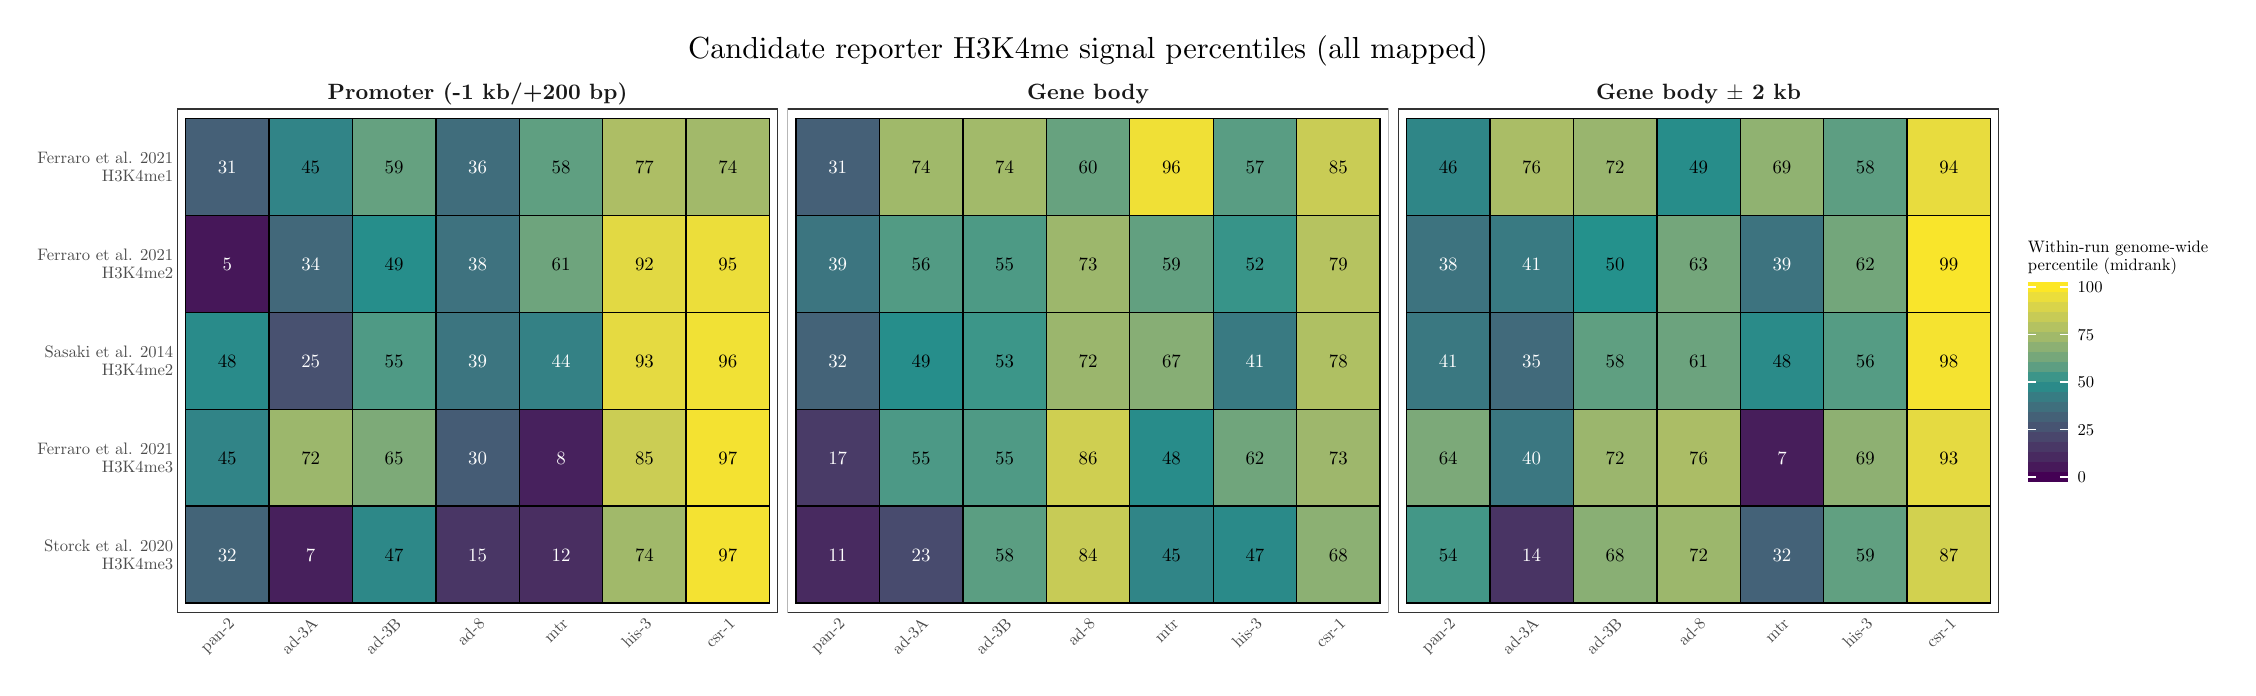
\begin{tikzpicture}[x=1pt,y=1pt]
\definecolor{fillColor}{RGB}{255,255,255}
\path[use as bounding box,fill=fillColor,fill opacity=0.00] (0,0) rectangle (794.97,231.26);
\begin{scope}
\path[clip] (  0.00,  0.00) rectangle (794.97,231.26);
\definecolor{drawColor}{RGB}{255,255,255}
\definecolor{fillColor}{RGB}{255,255,255}

\path[draw=drawColor,line width= 0.7pt,line join=round,line cap=round,fill=fillColor] (  0.00,  0.00) rectangle (794.97,231.26);
\end{scope}
\begin{scope}
\path[clip] ( 54.02, 19.84) rectangle (271.12,201.87);
\definecolor{fillColor}{RGB}{255,255,255}

\path[fill=fillColor] ( 54.02, 19.84) rectangle (271.12,201.87);
\definecolor{drawColor}{RGB}{0,0,0}
\definecolor{fillColor}{RGB}{69,96,119}

\path[draw=drawColor,line width= 0.5pt,fill=fillColor] ( 57.04,163.37) rectangle ( 87.19,198.37);
\definecolor{fillColor}{RGB}{49,132,135}

\path[draw=drawColor,line width= 0.5pt,fill=fillColor] ( 87.19,163.37) rectangle (117.34,198.37);
\definecolor{fillColor}{RGB}{101,161,128}

\path[draw=drawColor,line width= 0.5pt,fill=fillColor] (117.34,163.37) rectangle (147.49,198.37);
\definecolor{fillColor}{RGB}{64,109,124}

\path[draw=drawColor,line width= 0.5pt,fill=fillColor] (147.49,163.37) rectangle (177.64,198.37);
\definecolor{fillColor}{RGB}{95,159,129}

\path[draw=drawColor,line width= 0.5pt,fill=fillColor] (177.64,163.37) rectangle (207.80,198.37);
\definecolor{fillColor}{RGB}{173,190,101}

\path[draw=drawColor,line width= 0.5pt,fill=fillColor] (207.80,163.37) rectangle (237.95,198.37);
\definecolor{fillColor}{RGB}{162,185,106}

\path[draw=drawColor,line width= 0.5pt,fill=fillColor] (237.95,163.37) rectangle (268.10,198.37);
\definecolor{fillColor}{RGB}{70,23,89}

\path[draw=drawColor,line width= 0.5pt,fill=fillColor] ( 57.04,128.36) rectangle ( 87.19,163.37);
\definecolor{fillColor}{RGB}{66,104,122}

\path[draw=drawColor,line width= 0.5pt,fill=fillColor] ( 87.19,128.36) rectangle (117.34,163.37);
\definecolor{fillColor}{RGB}{38,142,139}

\path[draw=drawColor,line width= 0.5pt,fill=fillColor] (117.34,128.36) rectangle (147.49,163.37);
\definecolor{fillColor}{RGB}{62,114,127}

\path[draw=drawColor,line width= 0.5pt,fill=fillColor] (147.49,128.36) rectangle (177.64,163.37);
\definecolor{fillColor}{RGB}{110,164,125}

\path[draw=drawColor,line width= 0.5pt,fill=fillColor] (177.64,128.36) rectangle (207.80,163.37);
\definecolor{fillColor}{RGB}{226,217,67}

\path[draw=drawColor,line width= 0.5pt,fill=fillColor] (207.80,128.36) rectangle (237.95,163.37);
\definecolor{fillColor}{RGB}{236,222,58}

\path[draw=drawColor,line width= 0.5pt,fill=fillColor] (237.95,128.36) rectangle (268.10,163.37);
\definecolor{fillColor}{RGB}{41,139,138}

\path[draw=drawColor,line width= 0.5pt,fill=fillColor] ( 57.04, 93.35) rectangle ( 87.19,128.36);
\definecolor{fillColor}{RGB}{72,81,112}

\path[draw=drawColor,line width= 0.5pt,fill=fillColor] ( 87.19, 93.35) rectangle (117.34,128.36);
\definecolor{fillColor}{RGB}{79,154,133}

\path[draw=drawColor,line width= 0.5pt,fill=fillColor] (117.34, 93.35) rectangle (147.49,128.36);
\definecolor{fillColor}{RGB}{60,117,128}

\path[draw=drawColor,line width= 0.5pt,fill=fillColor] (147.49, 93.35) rectangle (177.64,128.36);
\definecolor{fillColor}{RGB}{52,129,133}

\path[draw=drawColor,line width= 0.5pt,fill=fillColor] (177.64, 93.35) rectangle (207.80,128.36);
\definecolor{fillColor}{RGB}{229,218,65}

\path[draw=drawColor,line width= 0.5pt,fill=fillColor] (207.80, 93.35) rectangle (237.95,128.36);
\definecolor{fillColor}{RGB}{241,225,53}

\path[draw=drawColor,line width= 0.5pt,fill=fillColor] (237.95, 93.35) rectangle (268.10,128.36);
\definecolor{fillColor}{RGB}{49,132,135}

\path[draw=drawColor,line width= 0.5pt,fill=fillColor] ( 57.04, 58.35) rectangle ( 87.19, 93.35);
\definecolor{fillColor}{RGB}{156,183,108}

\path[draw=drawColor,line width= 0.5pt,fill=fillColor] ( 87.19, 58.35) rectangle (117.34, 93.35);
\definecolor{fillColor}{RGB}{125,170,120}

\path[draw=drawColor,line width= 0.5pt,fill=fillColor] (117.34, 58.35) rectangle (147.49, 93.35);
\definecolor{fillColor}{RGB}{69,92,117}

\path[draw=drawColor,line width= 0.5pt,fill=fillColor] (147.49, 58.35) rectangle (177.64, 93.35);
\definecolor{fillColor}{RGB}{71,33,93}

\path[draw=drawColor,line width= 0.5pt,fill=fillColor] (177.64, 58.35) rectangle (207.80, 93.35);
\definecolor{fillColor}{RGB}{203,205,84}

\path[draw=drawColor,line width= 0.5pt,fill=fillColor] (207.80, 58.35) rectangle (237.95, 93.35);
\definecolor{fillColor}{RGB}{244,226,49}

\path[draw=drawColor,line width= 0.5pt,fill=fillColor] (237.95, 58.35) rectangle (268.10, 93.35);
\definecolor{fillColor}{RGB}{67,100,120}

\path[draw=drawColor,line width= 0.5pt,fill=fillColor] ( 57.04, 23.34) rectangle ( 87.19, 58.35);
\definecolor{fillColor}{RGB}{71,32,92}

\path[draw=drawColor,line width= 0.5pt,fill=fillColor] ( 87.19, 23.34) rectangle (117.34, 58.35);
\definecolor{fillColor}{RGB}{45,136,136}

\path[draw=drawColor,line width= 0.5pt,fill=fillColor] (117.34, 23.34) rectangle (147.49, 58.35);
\definecolor{fillColor}{RGB}{73,54,101}

\path[draw=drawColor,line width= 0.5pt,fill=fillColor] (147.49, 23.34) rectangle (177.64, 58.35);
\definecolor{fillColor}{RGB}{73,46,97}

\path[draw=drawColor,line width= 0.5pt,fill=fillColor] (177.64, 23.34) rectangle (207.80, 58.35);
\definecolor{fillColor}{RGB}{161,185,106}

\path[draw=drawColor,line width= 0.5pt,fill=fillColor] (207.80, 23.34) rectangle (237.95, 58.35);
\definecolor{fillColor}{RGB}{244,226,50}

\path[draw=drawColor,line width= 0.5pt,fill=fillColor] (237.95, 23.34) rectangle (268.10, 58.35);
\definecolor{drawColor}{RGB}{255,255,255}

\node[text=drawColor,anchor=base,inner sep=0pt, outer sep=0pt, scale=  0.68] at ( 72.11,178.52) {31};
\definecolor{drawColor}{RGB}{0,0,0}

\node[text=drawColor,anchor=base,inner sep=0pt, outer sep=0pt, scale=  0.68] at (102.26,178.52) {45};

\node[text=drawColor,anchor=base,inner sep=0pt, outer sep=0pt, scale=  0.68] at (132.42,178.52) {59};
\definecolor{drawColor}{RGB}{255,255,255}

\node[text=drawColor,anchor=base,inner sep=0pt, outer sep=0pt, scale=  0.68] at (162.57,178.52) {36};
\definecolor{drawColor}{RGB}{0,0,0}

\node[text=drawColor,anchor=base,inner sep=0pt, outer sep=0pt, scale=  0.68] at (192.72,178.52) {58};

\node[text=drawColor,anchor=base,inner sep=0pt, outer sep=0pt, scale=  0.68] at (222.87,178.52) {77};

\node[text=drawColor,anchor=base,inner sep=0pt, outer sep=0pt, scale=  0.68] at (253.02,178.52) {74};
\definecolor{drawColor}{RGB}{255,255,255}

\node[text=drawColor,anchor=base,inner sep=0pt, outer sep=0pt, scale=  0.68] at ( 72.11,143.51) {5};

\node[text=drawColor,anchor=base,inner sep=0pt, outer sep=0pt, scale=  0.68] at (102.26,143.51) {34};
\definecolor{drawColor}{RGB}{0,0,0}

\node[text=drawColor,anchor=base,inner sep=0pt, outer sep=0pt, scale=  0.68] at (132.42,143.51) {49};
\definecolor{drawColor}{RGB}{255,255,255}

\node[text=drawColor,anchor=base,inner sep=0pt, outer sep=0pt, scale=  0.68] at (162.57,143.51) {38};
\definecolor{drawColor}{RGB}{0,0,0}

\node[text=drawColor,anchor=base,inner sep=0pt, outer sep=0pt, scale=  0.68] at (192.72,143.51) {61};

\node[text=drawColor,anchor=base,inner sep=0pt, outer sep=0pt, scale=  0.68] at (222.87,143.51) {92};

\node[text=drawColor,anchor=base,inner sep=0pt, outer sep=0pt, scale=  0.68] at (253.02,143.51) {95};

\node[text=drawColor,anchor=base,inner sep=0pt, outer sep=0pt, scale=  0.68] at ( 72.11,108.51) {48};
\definecolor{drawColor}{RGB}{255,255,255}

\node[text=drawColor,anchor=base,inner sep=0pt, outer sep=0pt, scale=  0.68] at (102.26,108.51) {25};
\definecolor{drawColor}{RGB}{0,0,0}

\node[text=drawColor,anchor=base,inner sep=0pt, outer sep=0pt, scale=  0.68] at (132.42,108.51) {55};
\definecolor{drawColor}{RGB}{255,255,255}

\node[text=drawColor,anchor=base,inner sep=0pt, outer sep=0pt, scale=  0.68] at (162.57,108.51) {39};

\node[text=drawColor,anchor=base,inner sep=0pt, outer sep=0pt, scale=  0.68] at (192.72,108.51) {44};
\definecolor{drawColor}{RGB}{0,0,0}

\node[text=drawColor,anchor=base,inner sep=0pt, outer sep=0pt, scale=  0.68] at (222.87,108.51) {93};

\node[text=drawColor,anchor=base,inner sep=0pt, outer sep=0pt, scale=  0.68] at (253.02,108.51) {96};

\node[text=drawColor,anchor=base,inner sep=0pt, outer sep=0pt, scale=  0.68] at ( 72.11, 73.50) {45};

\node[text=drawColor,anchor=base,inner sep=0pt, outer sep=0pt, scale=  0.68] at (102.26, 73.50) {72};

\node[text=drawColor,anchor=base,inner sep=0pt, outer sep=0pt, scale=  0.68] at (132.42, 73.50) {65};
\definecolor{drawColor}{RGB}{255,255,255}

\node[text=drawColor,anchor=base,inner sep=0pt, outer sep=0pt, scale=  0.68] at (162.57, 73.50) {30};

\node[text=drawColor,anchor=base,inner sep=0pt, outer sep=0pt, scale=  0.68] at (192.72, 73.50) {8};
\definecolor{drawColor}{RGB}{0,0,0}

\node[text=drawColor,anchor=base,inner sep=0pt, outer sep=0pt, scale=  0.68] at (222.87, 73.50) {85};

\node[text=drawColor,anchor=base,inner sep=0pt, outer sep=0pt, scale=  0.68] at (253.02, 73.50) {97};
\definecolor{drawColor}{RGB}{255,255,255}

\node[text=drawColor,anchor=base,inner sep=0pt, outer sep=0pt, scale=  0.68] at ( 72.11, 38.49) {32};

\node[text=drawColor,anchor=base,inner sep=0pt, outer sep=0pt, scale=  0.68] at (102.26, 38.49) {7};
\definecolor{drawColor}{RGB}{0,0,0}

\node[text=drawColor,anchor=base,inner sep=0pt, outer sep=0pt, scale=  0.68] at (132.42, 38.49) {47};
\definecolor{drawColor}{RGB}{255,255,255}

\node[text=drawColor,anchor=base,inner sep=0pt, outer sep=0pt, scale=  0.68] at (162.57, 38.49) {15};

\node[text=drawColor,anchor=base,inner sep=0pt, outer sep=0pt, scale=  0.68] at (192.72, 38.49) {12};
\definecolor{drawColor}{RGB}{0,0,0}

\node[text=drawColor,anchor=base,inner sep=0pt, outer sep=0pt, scale=  0.68] at (222.87, 38.49) {74};

\node[text=drawColor,anchor=base,inner sep=0pt, outer sep=0pt, scale=  0.68] at (253.02, 38.49) {97};
\definecolor{drawColor}{gray}{0.20}

\path[draw=drawColor,line width= 0.6pt,line join=round,line cap=round] ( 54.02, 19.84) rectangle (271.12,201.87);
\end{scope}
\begin{scope}
\path[clip] (274.62, 19.84) rectangle (491.71,201.87);
\definecolor{fillColor}{RGB}{255,255,255}

\path[fill=fillColor] (274.62, 19.84) rectangle (491.71,201.87);
\definecolor{drawColor}{RGB}{0,0,0}
\definecolor{fillColor}{RGB}{69,96,119}

\path[draw=drawColor,line width= 0.5pt,fill=fillColor] (277.63,163.37) rectangle (307.78,198.37);
\definecolor{fillColor}{RGB}{160,185,106}

\path[draw=drawColor,line width= 0.5pt,fill=fillColor] (307.78,163.37) rectangle (337.93,198.37);
\definecolor{fillColor}{RGB}{162,186,106}

\path[draw=drawColor,line width= 0.5pt,fill=fillColor] (337.93,163.37) rectangle (368.09,198.37);
\definecolor{fillColor}{RGB}{103,162,127}

\path[draw=drawColor,line width= 0.5pt,fill=fillColor] (368.09,163.37) rectangle (398.24,198.37);
\definecolor{fillColor}{RGB}{240,224,54}

\path[draw=drawColor,line width= 0.5pt,fill=fillColor] (398.24,163.37) rectangle (428.39,198.37);
\definecolor{fillColor}{RGB}{89,157,131}

\path[draw=drawColor,line width= 0.5pt,fill=fillColor] (428.39,163.37) rectangle (458.54,198.37);
\definecolor{fillColor}{RGB}{201,204,85}

\path[draw=drawColor,line width= 0.5pt,fill=fillColor] (458.54,163.37) rectangle (488.69,198.37);
\definecolor{fillColor}{RGB}{60,117,128}

\path[draw=drawColor,line width= 0.5pt,fill=fillColor] (277.63,128.36) rectangle (307.78,163.37);
\definecolor{fillColor}{RGB}{82,155,132}

\path[draw=drawColor,line width= 0.5pt,fill=fillColor] (307.78,128.36) rectangle (337.93,163.37);
\definecolor{fillColor}{RGB}{77,154,133}

\path[draw=drawColor,line width= 0.5pt,fill=fillColor] (337.93,128.36) rectangle (368.09,163.37);
\definecolor{fillColor}{RGB}{157,183,108}

\path[draw=drawColor,line width= 0.5pt,fill=fillColor] (368.09,128.36) rectangle (398.24,163.37);
\definecolor{fillColor}{RGB}{98,160,128}

\path[draw=drawColor,line width= 0.5pt,fill=fillColor] (398.24,128.36) rectangle (428.39,163.37);
\definecolor{fillColor}{RGB}{55,148,137}

\path[draw=drawColor,line width= 0.5pt,fill=fillColor] (428.39,128.36) rectangle (458.54,163.37);
\definecolor{fillColor}{RGB}{182,195,96}

\path[draw=drawColor,line width= 0.5pt,fill=fillColor] (458.54,128.36) rectangle (488.69,163.37);
\definecolor{fillColor}{RGB}{68,99,120}

\path[draw=drawColor,line width= 0.5pt,fill=fillColor] (277.63, 93.35) rectangle (307.78,128.36);
\definecolor{fillColor}{RGB}{38,142,139}

\path[draw=drawColor,line width= 0.5pt,fill=fillColor] (307.78, 93.35) rectangle (337.93,128.36);
\definecolor{fillColor}{RGB}{60,150,137}

\path[draw=drawColor,line width= 0.5pt,fill=fillColor] (337.93, 93.35) rectangle (368.09,128.36);
\definecolor{fillColor}{RGB}{155,182,109}

\path[draw=drawColor,line width= 0.5pt,fill=fillColor] (368.09, 93.35) rectangle (398.24,128.36);
\definecolor{fillColor}{RGB}{135,174,117}

\path[draw=drawColor,line width= 0.5pt,fill=fillColor] (398.24, 93.35) rectangle (428.39,128.36);
\definecolor{fillColor}{RGB}{57,122,130}

\path[draw=drawColor,line width= 0.5pt,fill=fillColor] (428.39, 93.35) rectangle (458.54,128.36);
\definecolor{fillColor}{RGB}{175,192,99}

\path[draw=drawColor,line width= 0.5pt,fill=fillColor] (458.54, 93.35) rectangle (488.69,128.36);
\definecolor{fillColor}{RGB}{73,59,103}

\path[draw=drawColor,line width= 0.5pt,fill=fillColor] (277.63, 58.35) rectangle (307.78, 93.35);
\definecolor{fillColor}{RGB}{76,153,134}

\path[draw=drawColor,line width= 0.5pt,fill=fillColor] (307.78, 58.35) rectangle (337.93, 93.35);
\definecolor{fillColor}{RGB}{79,154,133}

\path[draw=drawColor,line width= 0.5pt,fill=fillColor] (337.93, 58.35) rectangle (368.09, 93.35);
\definecolor{fillColor}{RGB}{207,207,81}

\path[draw=drawColor,line width= 0.5pt,fill=fillColor] (368.09, 58.35) rectangle (398.24, 93.35);
\definecolor{fillColor}{RGB}{40,140,138}

\path[draw=drawColor,line width= 0.5pt,fill=fillColor] (398.24, 58.35) rectangle (428.39, 93.35);
\definecolor{fillColor}{RGB}{112,165,124}

\path[draw=drawColor,line width= 0.5pt,fill=fillColor] (428.39, 58.35) rectangle (458.54, 93.35);
\definecolor{fillColor}{RGB}{158,183,108}

\path[draw=drawColor,line width= 0.5pt,fill=fillColor] (458.54, 58.35) rectangle (488.69, 93.35);
\definecolor{fillColor}{RGB}{72,42,96}

\path[draw=drawColor,line width= 0.5pt,fill=fillColor] (277.63, 23.34) rectangle (307.78, 58.35);
\definecolor{fillColor}{RGB}{72,75,110}

\path[draw=drawColor,line width= 0.5pt,fill=fillColor] (307.78, 23.34) rectangle (337.93, 58.35);
\definecolor{fillColor}{RGB}{91,158,130}

\path[draw=drawColor,line width= 0.5pt,fill=fillColor] (337.93, 23.34) rectangle (368.09, 58.35);
\definecolor{fillColor}{RGB}{199,203,86}

\path[draw=drawColor,line width= 0.5pt,fill=fillColor] (368.09, 23.34) rectangle (398.24, 58.35);
\definecolor{fillColor}{RGB}{48,133,135}

\path[draw=drawColor,line width= 0.5pt,fill=fillColor] (398.24, 23.34) rectangle (428.39, 58.35);
\definecolor{fillColor}{RGB}{42,138,137}

\path[draw=drawColor,line width= 0.5pt,fill=fillColor] (428.39, 23.34) rectangle (458.54, 58.35);
\definecolor{fillColor}{RGB}{140,176,115}

\path[draw=drawColor,line width= 0.5pt,fill=fillColor] (458.54, 23.34) rectangle (488.69, 58.35);
\definecolor{drawColor}{RGB}{255,255,255}

\node[text=drawColor,anchor=base,inner sep=0pt, outer sep=0pt, scale=  0.68] at (292.71,178.52) {31};
\definecolor{drawColor}{RGB}{0,0,0}

\node[text=drawColor,anchor=base,inner sep=0pt, outer sep=0pt, scale=  0.68] at (322.86,178.52) {74};

\node[text=drawColor,anchor=base,inner sep=0pt, outer sep=0pt, scale=  0.68] at (353.01,178.52) {74};

\node[text=drawColor,anchor=base,inner sep=0pt, outer sep=0pt, scale=  0.68] at (383.16,178.52) {60};

\node[text=drawColor,anchor=base,inner sep=0pt, outer sep=0pt, scale=  0.68] at (413.31,178.52) {96};

\node[text=drawColor,anchor=base,inner sep=0pt, outer sep=0pt, scale=  0.68] at (443.47,178.52) {57};

\node[text=drawColor,anchor=base,inner sep=0pt, outer sep=0pt, scale=  0.68] at (473.62,178.52) {85};
\definecolor{drawColor}{RGB}{255,255,255}

\node[text=drawColor,anchor=base,inner sep=0pt, outer sep=0pt, scale=  0.68] at (292.71,143.51) {39};
\definecolor{drawColor}{RGB}{0,0,0}

\node[text=drawColor,anchor=base,inner sep=0pt, outer sep=0pt, scale=  0.68] at (322.86,143.51) {56};

\node[text=drawColor,anchor=base,inner sep=0pt, outer sep=0pt, scale=  0.68] at (353.01,143.51) {55};

\node[text=drawColor,anchor=base,inner sep=0pt, outer sep=0pt, scale=  0.68] at (383.16,143.51) {73};

\node[text=drawColor,anchor=base,inner sep=0pt, outer sep=0pt, scale=  0.68] at (413.31,143.51) {59};

\node[text=drawColor,anchor=base,inner sep=0pt, outer sep=0pt, scale=  0.68] at (443.47,143.51) {52};

\node[text=drawColor,anchor=base,inner sep=0pt, outer sep=0pt, scale=  0.68] at (473.62,143.51) {79};
\definecolor{drawColor}{RGB}{255,255,255}

\node[text=drawColor,anchor=base,inner sep=0pt, outer sep=0pt, scale=  0.68] at (292.71,108.51) {32};
\definecolor{drawColor}{RGB}{0,0,0}

\node[text=drawColor,anchor=base,inner sep=0pt, outer sep=0pt, scale=  0.68] at (322.86,108.51) {49};

\node[text=drawColor,anchor=base,inner sep=0pt, outer sep=0pt, scale=  0.68] at (353.01,108.51) {53};

\node[text=drawColor,anchor=base,inner sep=0pt, outer sep=0pt, scale=  0.68] at (383.16,108.51) {72};

\node[text=drawColor,anchor=base,inner sep=0pt, outer sep=0pt, scale=  0.68] at (413.31,108.51) {67};
\definecolor{drawColor}{RGB}{255,255,255}

\node[text=drawColor,anchor=base,inner sep=0pt, outer sep=0pt, scale=  0.68] at (443.47,108.51) {41};
\definecolor{drawColor}{RGB}{0,0,0}

\node[text=drawColor,anchor=base,inner sep=0pt, outer sep=0pt, scale=  0.68] at (473.62,108.51) {78};
\definecolor{drawColor}{RGB}{255,255,255}

\node[text=drawColor,anchor=base,inner sep=0pt, outer sep=0pt, scale=  0.68] at (292.71, 73.50) {17};
\definecolor{drawColor}{RGB}{0,0,0}

\node[text=drawColor,anchor=base,inner sep=0pt, outer sep=0pt, scale=  0.68] at (322.86, 73.50) {55};

\node[text=drawColor,anchor=base,inner sep=0pt, outer sep=0pt, scale=  0.68] at (353.01, 73.50) {55};

\node[text=drawColor,anchor=base,inner sep=0pt, outer sep=0pt, scale=  0.68] at (383.16, 73.50) {86};

\node[text=drawColor,anchor=base,inner sep=0pt, outer sep=0pt, scale=  0.68] at (413.31, 73.50) {48};

\node[text=drawColor,anchor=base,inner sep=0pt, outer sep=0pt, scale=  0.68] at (443.47, 73.50) {62};

\node[text=drawColor,anchor=base,inner sep=0pt, outer sep=0pt, scale=  0.68] at (473.62, 73.50) {73};
\definecolor{drawColor}{RGB}{255,255,255}

\node[text=drawColor,anchor=base,inner sep=0pt, outer sep=0pt, scale=  0.68] at (292.71, 38.49) {11};

\node[text=drawColor,anchor=base,inner sep=0pt, outer sep=0pt, scale=  0.68] at (322.86, 38.49) {23};
\definecolor{drawColor}{RGB}{0,0,0}

\node[text=drawColor,anchor=base,inner sep=0pt, outer sep=0pt, scale=  0.68] at (353.01, 38.49) {58};

\node[text=drawColor,anchor=base,inner sep=0pt, outer sep=0pt, scale=  0.68] at (383.16, 38.49) {84};

\node[text=drawColor,anchor=base,inner sep=0pt, outer sep=0pt, scale=  0.68] at (413.31, 38.49) {45};

\node[text=drawColor,anchor=base,inner sep=0pt, outer sep=0pt, scale=  0.68] at (443.47, 38.49) {47};

\node[text=drawColor,anchor=base,inner sep=0pt, outer sep=0pt, scale=  0.68] at (473.62, 38.49) {68};
\definecolor{drawColor}{gray}{0.20}

\path[draw=drawColor,line width= 0.6pt,line join=round,line cap=round] (274.62, 19.84) rectangle (491.71,201.87);
\end{scope}
\begin{scope}
\path[clip] (495.21, 19.84) rectangle (712.30,201.87);
\definecolor{fillColor}{RGB}{255,255,255}

\path[fill=fillColor] (495.21, 19.84) rectangle (712.30,201.87);
\definecolor{drawColor}{RGB}{0,0,0}
\definecolor{fillColor}{RGB}{47,134,135}

\path[draw=drawColor,line width= 0.5pt,fill=fillColor] (498.22,163.37) rectangle (528.38,198.37);
\definecolor{fillColor}{RGB}{170,189,102}

\path[draw=drawColor,line width= 0.5pt,fill=fillColor] (528.38,163.37) rectangle (558.53,198.37);
\definecolor{fillColor}{RGB}{153,181,110}

\path[draw=drawColor,line width= 0.5pt,fill=fillColor] (558.53,163.37) rectangle (588.68,198.37);
\definecolor{fillColor}{RGB}{39,141,138}

\path[draw=drawColor,line width= 0.5pt,fill=fillColor] (588.68,163.37) rectangle (618.83,198.37);
\definecolor{fillColor}{RGB}{144,178,113}

\path[draw=drawColor,line width= 0.5pt,fill=fillColor] (618.83,163.37) rectangle (648.98,198.37);
\definecolor{fillColor}{RGB}{93,158,130}

\path[draw=drawColor,line width= 0.5pt,fill=fillColor] (648.98,163.37) rectangle (679.13,198.37);
\definecolor{fillColor}{RGB}{232,220,62}

\path[draw=drawColor,line width= 0.5pt,fill=fillColor] (679.13,163.37) rectangle (709.29,198.37);
\definecolor{fillColor}{RGB}{61,115,127}

\path[draw=drawColor,line width= 0.5pt,fill=fillColor] (498.22,128.36) rectangle (528.38,163.37);
\definecolor{fillColor}{RGB}{57,122,130}

\path[draw=drawColor,line width= 0.5pt,fill=fillColor] (528.38,128.36) rectangle (558.53,163.37);
\definecolor{fillColor}{RGB}{36,145,140}

\path[draw=drawColor,line width= 0.5pt,fill=fillColor] (558.53,128.36) rectangle (588.68,163.37);
\definecolor{fillColor}{RGB}{116,166,123}

\path[draw=drawColor,line width= 0.5pt,fill=fillColor] (588.68,128.36) rectangle (618.83,163.37);
\definecolor{fillColor}{RGB}{61,115,127}

\path[draw=drawColor,line width= 0.5pt,fill=fillColor] (618.83,128.36) rectangle (648.98,163.37);
\definecolor{fillColor}{RGB}{115,166,123}

\path[draw=drawColor,line width= 0.5pt,fill=fillColor] (648.98,128.36) rectangle (679.13,163.37);
\definecolor{fillColor}{RGB}{249,229,43}

\path[draw=drawColor,line width= 0.5pt,fill=fillColor] (679.13,128.36) rectangle (709.29,163.37);
\definecolor{fillColor}{RGB}{58,120,129}

\path[draw=drawColor,line width= 0.5pt,fill=fillColor] (498.22, 93.35) rectangle (528.38,128.36);
\definecolor{fillColor}{RGB}{65,106,123}

\path[draw=drawColor,line width= 0.5pt,fill=fillColor] (528.38, 93.35) rectangle (558.53,128.36);
\definecolor{fillColor}{RGB}{95,159,129}

\path[draw=drawColor,line width= 0.5pt,fill=fillColor] (558.53, 93.35) rectangle (588.68,128.36);
\definecolor{fillColor}{RGB}{108,163,126}

\path[draw=drawColor,line width= 0.5pt,fill=fillColor] (588.68, 93.35) rectangle (618.83,128.36);
\definecolor{fillColor}{RGB}{42,139,137}

\path[draw=drawColor,line width= 0.5pt,fill=fillColor] (618.83, 93.35) rectangle (648.98,128.36);
\definecolor{fillColor}{RGB}{85,156,132}

\path[draw=drawColor,line width= 0.5pt,fill=fillColor] (648.98, 93.35) rectangle (679.13,128.36);
\definecolor{fillColor}{RGB}{245,227,48}

\path[draw=drawColor,line width= 0.5pt,fill=fillColor] (679.13, 93.35) rectangle (709.29,128.36);
\definecolor{fillColor}{RGB}{124,169,121}

\path[draw=drawColor,line width= 0.5pt,fill=fillColor] (498.22, 58.35) rectangle (528.38, 93.35);
\definecolor{fillColor}{RGB}{59,119,129}

\path[draw=drawColor,line width= 0.5pt,fill=fillColor] (528.38, 58.35) rectangle (558.53, 93.35);
\definecolor{fillColor}{RGB}{155,182,109}

\path[draw=drawColor,line width= 0.5pt,fill=fillColor] (558.53, 58.35) rectangle (588.68, 93.35);
\definecolor{fillColor}{RGB}{171,189,102}

\path[draw=drawColor,line width= 0.5pt,fill=fillColor] (588.68, 58.35) rectangle (618.83, 93.35);
\definecolor{fillColor}{RGB}{71,30,91}

\path[draw=drawColor,line width= 0.5pt,fill=fillColor] (618.83, 58.35) rectangle (648.98, 93.35);
\definecolor{fillColor}{RGB}{142,176,114}

\path[draw=drawColor,line width= 0.5pt,fill=fillColor] (648.98, 58.35) rectangle (679.13, 93.35);
\definecolor{fillColor}{RGB}{229,218,65}

\path[draw=drawColor,line width= 0.5pt,fill=fillColor] (679.13, 58.35) rectangle (709.29, 93.35);
\definecolor{fillColor}{RGB}{67,151,135}

\path[draw=drawColor,line width= 0.5pt,fill=fillColor] (498.22, 23.34) rectangle (528.38, 58.35);
\definecolor{fillColor}{RGB}{73,52,100}

\path[draw=drawColor,line width= 0.5pt,fill=fillColor] (528.38, 23.34) rectangle (558.53, 58.35);
\definecolor{fillColor}{RGB}{137,175,116}

\path[draw=drawColor,line width= 0.5pt,fill=fillColor] (558.53, 23.34) rectangle (588.68, 58.35);
\definecolor{fillColor}{RGB}{156,183,108}

\path[draw=drawColor,line width= 0.5pt,fill=fillColor] (588.68, 23.34) rectangle (618.83, 58.35);
\definecolor{fillColor}{RGB}{68,98,120}

\path[draw=drawColor,line width= 0.5pt,fill=fillColor] (618.83, 23.34) rectangle (648.98, 58.35);
\definecolor{fillColor}{RGB}{97,160,129}

\path[draw=drawColor,line width= 0.5pt,fill=fillColor] (648.98, 23.34) rectangle (679.13, 58.35);
\definecolor{fillColor}{RGB}{210,209,79}

\path[draw=drawColor,line width= 0.5pt,fill=fillColor] (679.13, 23.34) rectangle (709.29, 58.35);

\node[text=drawColor,anchor=base,inner sep=0pt, outer sep=0pt, scale=  0.68] at (513.30,178.52) {46};

\node[text=drawColor,anchor=base,inner sep=0pt, outer sep=0pt, scale=  0.68] at (543.45,178.52) {76};

\node[text=drawColor,anchor=base,inner sep=0pt, outer sep=0pt, scale=  0.68] at (573.60,178.52) {72};

\node[text=drawColor,anchor=base,inner sep=0pt, outer sep=0pt, scale=  0.68] at (603.76,178.52) {49};

\node[text=drawColor,anchor=base,inner sep=0pt, outer sep=0pt, scale=  0.68] at (633.91,178.52) {69};

\node[text=drawColor,anchor=base,inner sep=0pt, outer sep=0pt, scale=  0.68] at (664.06,178.52) {58};

\node[text=drawColor,anchor=base,inner sep=0pt, outer sep=0pt, scale=  0.68] at (694.21,178.52) {94};
\definecolor{drawColor}{RGB}{255,255,255}

\node[text=drawColor,anchor=base,inner sep=0pt, outer sep=0pt, scale=  0.68] at (513.30,143.51) {38};

\node[text=drawColor,anchor=base,inner sep=0pt, outer sep=0pt, scale=  0.68] at (543.45,143.51) {41};
\definecolor{drawColor}{RGB}{0,0,0}

\node[text=drawColor,anchor=base,inner sep=0pt, outer sep=0pt, scale=  0.68] at (573.60,143.51) {50};

\node[text=drawColor,anchor=base,inner sep=0pt, outer sep=0pt, scale=  0.68] at (603.76,143.51) {63};
\definecolor{drawColor}{RGB}{255,255,255}

\node[text=drawColor,anchor=base,inner sep=0pt, outer sep=0pt, scale=  0.68] at (633.91,143.51) {39};
\definecolor{drawColor}{RGB}{0,0,0}

\node[text=drawColor,anchor=base,inner sep=0pt, outer sep=0pt, scale=  0.68] at (664.06,143.51) {62};

\node[text=drawColor,anchor=base,inner sep=0pt, outer sep=0pt, scale=  0.68] at (694.21,143.51) {99};
\definecolor{drawColor}{RGB}{255,255,255}

\node[text=drawColor,anchor=base,inner sep=0pt, outer sep=0pt, scale=  0.68] at (513.30,108.51) {41};

\node[text=drawColor,anchor=base,inner sep=0pt, outer sep=0pt, scale=  0.68] at (543.45,108.51) {35};
\definecolor{drawColor}{RGB}{0,0,0}

\node[text=drawColor,anchor=base,inner sep=0pt, outer sep=0pt, scale=  0.68] at (573.60,108.51) {58};

\node[text=drawColor,anchor=base,inner sep=0pt, outer sep=0pt, scale=  0.68] at (603.76,108.51) {61};

\node[text=drawColor,anchor=base,inner sep=0pt, outer sep=0pt, scale=  0.68] at (633.91,108.51) {48};

\node[text=drawColor,anchor=base,inner sep=0pt, outer sep=0pt, scale=  0.68] at (664.06,108.51) {56};

\node[text=drawColor,anchor=base,inner sep=0pt, outer sep=0pt, scale=  0.68] at (694.21,108.51) {98};

\node[text=drawColor,anchor=base,inner sep=0pt, outer sep=0pt, scale=  0.68] at (513.30, 73.50) {64};
\definecolor{drawColor}{RGB}{255,255,255}

\node[text=drawColor,anchor=base,inner sep=0pt, outer sep=0pt, scale=  0.68] at (543.45, 73.50) {40};
\definecolor{drawColor}{RGB}{0,0,0}

\node[text=drawColor,anchor=base,inner sep=0pt, outer sep=0pt, scale=  0.68] at (573.60, 73.50) {72};

\node[text=drawColor,anchor=base,inner sep=0pt, outer sep=0pt, scale=  0.68] at (603.76, 73.50) {76};
\definecolor{drawColor}{RGB}{255,255,255}

\node[text=drawColor,anchor=base,inner sep=0pt, outer sep=0pt, scale=  0.68] at (633.91, 73.50) {7};
\definecolor{drawColor}{RGB}{0,0,0}

\node[text=drawColor,anchor=base,inner sep=0pt, outer sep=0pt, scale=  0.68] at (664.06, 73.50) {69};

\node[text=drawColor,anchor=base,inner sep=0pt, outer sep=0pt, scale=  0.68] at (694.21, 73.50) {93};

\node[text=drawColor,anchor=base,inner sep=0pt, outer sep=0pt, scale=  0.68] at (513.30, 38.49) {54};
\definecolor{drawColor}{RGB}{255,255,255}

\node[text=drawColor,anchor=base,inner sep=0pt, outer sep=0pt, scale=  0.68] at (543.45, 38.49) {14};
\definecolor{drawColor}{RGB}{0,0,0}

\node[text=drawColor,anchor=base,inner sep=0pt, outer sep=0pt, scale=  0.68] at (573.60, 38.49) {68};

\node[text=drawColor,anchor=base,inner sep=0pt, outer sep=0pt, scale=  0.68] at (603.76, 38.49) {72};
\definecolor{drawColor}{RGB}{255,255,255}

\node[text=drawColor,anchor=base,inner sep=0pt, outer sep=0pt, scale=  0.68] at (633.91, 38.49) {32};
\definecolor{drawColor}{RGB}{0,0,0}

\node[text=drawColor,anchor=base,inner sep=0pt, outer sep=0pt, scale=  0.68] at (664.06, 38.49) {59};

\node[text=drawColor,anchor=base,inner sep=0pt, outer sep=0pt, scale=  0.68] at (694.21, 38.49) {87};
\definecolor{drawColor}{gray}{0.20}

\path[draw=drawColor,line width= 0.6pt,line join=round,line cap=round] (495.21, 19.84) rectangle (712.30,201.87);
\end{scope}
\begin{scope}
\path[clip] ( 54.02,201.87) rectangle (271.12,214.55);
\definecolor{drawColor}{gray}{0.10}

\node[text=drawColor,anchor=base,inner sep=0pt, outer sep=0pt, scale=  0.80] at (162.57,205.45) {\bfseries Promoter (-1 kb/+200 bp)};
\end{scope}
\begin{scope}
\path[clip] (274.62,201.87) rectangle (491.71,214.55);
\definecolor{drawColor}{gray}{0.10}

\node[text=drawColor,anchor=base,inner sep=0pt, outer sep=0pt, scale=  0.80] at (383.16,205.45) {\bfseries Gene body};
\end{scope}
\begin{scope}
\path[clip] (495.21,201.87) rectangle (712.30,214.55);
\definecolor{drawColor}{gray}{0.10}

\node[text=drawColor,anchor=base,inner sep=0pt, outer sep=0pt, scale=  0.80] at (603.76,205.45) {\bfseries Gene body $\pm$ 2 kb};
\end{scope}
\begin{scope}
\path[clip] (  0.00,  0.00) rectangle (794.97,231.26);
\definecolor{drawColor}{gray}{0.30}

\node[text=drawColor,rotate= 45.00,anchor=base east,inner sep=0pt, outer sep=0pt, scale=  0.60] at ( 75.03, 15.52) {pan-2};

\node[text=drawColor,rotate= 45.00,anchor=base east,inner sep=0pt, outer sep=0pt, scale=  0.60] at (105.19, 15.52) {ad-3A};

\node[text=drawColor,rotate= 45.00,anchor=base east,inner sep=0pt, outer sep=0pt, scale=  0.60] at (135.34, 15.52) {ad-3B};

\node[text=drawColor,rotate= 45.00,anchor=base east,inner sep=0pt, outer sep=0pt, scale=  0.60] at (165.49, 15.52) {ad-8};

\node[text=drawColor,rotate= 45.00,anchor=base east,inner sep=0pt, outer sep=0pt, scale=  0.60] at (195.64, 15.52) {mtr};

\node[text=drawColor,rotate= 45.00,anchor=base east,inner sep=0pt, outer sep=0pt, scale=  0.60] at (225.79, 15.52) {his-3};

\node[text=drawColor,rotate= 45.00,anchor=base east,inner sep=0pt, outer sep=0pt, scale=  0.60] at (255.95, 15.52) {csr-1};
\end{scope}
\begin{scope}
\path[clip] (  0.00,  0.00) rectangle (794.97,231.26);
\definecolor{drawColor}{gray}{0.30}

\node[text=drawColor,rotate= 45.00,anchor=base east,inner sep=0pt, outer sep=0pt, scale=  0.60] at (295.63, 15.52) {pan-2};

\node[text=drawColor,rotate= 45.00,anchor=base east,inner sep=0pt, outer sep=0pt, scale=  0.60] at (325.78, 15.52) {ad-3A};

\node[text=drawColor,rotate= 45.00,anchor=base east,inner sep=0pt, outer sep=0pt, scale=  0.60] at (355.93, 15.52) {ad-3B};

\node[text=drawColor,rotate= 45.00,anchor=base east,inner sep=0pt, outer sep=0pt, scale=  0.60] at (386.08, 15.52) {ad-8};

\node[text=drawColor,rotate= 45.00,anchor=base east,inner sep=0pt, outer sep=0pt, scale=  0.60] at (416.24, 15.52) {mtr};

\node[text=drawColor,rotate= 45.00,anchor=base east,inner sep=0pt, outer sep=0pt, scale=  0.60] at (446.39, 15.52) {his-3};

\node[text=drawColor,rotate= 45.00,anchor=base east,inner sep=0pt, outer sep=0pt, scale=  0.60] at (476.54, 15.52) {csr-1};
\end{scope}
\begin{scope}
\path[clip] (  0.00,  0.00) rectangle (794.97,231.26);
\definecolor{drawColor}{gray}{0.30}

\node[text=drawColor,rotate= 45.00,anchor=base east,inner sep=0pt, outer sep=0pt, scale=  0.60] at (516.22, 15.52) {pan-2};

\node[text=drawColor,rotate= 45.00,anchor=base east,inner sep=0pt, outer sep=0pt, scale=  0.60] at (546.37, 15.52) {ad-3A};

\node[text=drawColor,rotate= 45.00,anchor=base east,inner sep=0pt, outer sep=0pt, scale=  0.60] at (576.53, 15.52) {ad-3B};

\node[text=drawColor,rotate= 45.00,anchor=base east,inner sep=0pt, outer sep=0pt, scale=  0.60] at (606.68, 15.52) {ad-8};

\node[text=drawColor,rotate= 45.00,anchor=base east,inner sep=0pt, outer sep=0pt, scale=  0.60] at (636.83, 15.52) {mtr};

\node[text=drawColor,rotate= 45.00,anchor=base east,inner sep=0pt, outer sep=0pt, scale=  0.60] at (666.98, 15.52) {his-3};

\node[text=drawColor,rotate= 45.00,anchor=base east,inner sep=0pt, outer sep=0pt, scale=  0.60] at (697.13, 15.52) {csr-1};
\end{scope}
\begin{scope}
\path[clip] (  0.00,  0.00) rectangle (794.97,231.26);
\definecolor{drawColor}{gray}{0.30}

\node[text=drawColor,anchor=base east,inner sep=0pt, outer sep=0pt, scale=  0.60] at ( 52.62, 42.02) {Storck et al. 2020};

\node[text=drawColor,anchor=base east,inner sep=0pt, outer sep=0pt, scale=  0.60] at ( 52.62, 35.54) {H3K4me3};

\node[text=drawColor,anchor=base east,inner sep=0pt, outer sep=0pt, scale=  0.60] at ( 52.62, 77.02) {Ferraro et al. 2021};

\node[text=drawColor,anchor=base east,inner sep=0pt, outer sep=0pt, scale=  0.60] at ( 52.62, 70.54) {H3K4me3};

\node[text=drawColor,anchor=base east,inner sep=0pt, outer sep=0pt, scale=  0.60] at ( 52.62,112.03) {Sasaki et al. 2014};

\node[text=drawColor,anchor=base east,inner sep=0pt, outer sep=0pt, scale=  0.60] at ( 52.62,105.55) {H3K4me2};

\node[text=drawColor,anchor=base east,inner sep=0pt, outer sep=0pt, scale=  0.60] at ( 52.62,147.04) {Ferraro et al. 2021};

\node[text=drawColor,anchor=base east,inner sep=0pt, outer sep=0pt, scale=  0.60] at ( 52.62,140.56) {H3K4me2};

\node[text=drawColor,anchor=base east,inner sep=0pt, outer sep=0pt, scale=  0.60] at ( 52.62,182.04) {Ferraro et al. 2021};

\node[text=drawColor,anchor=base east,inner sep=0pt, outer sep=0pt, scale=  0.60] at ( 52.62,175.56) {H3K4me1};
\end{scope}
\begin{scope}
\path[clip] (  0.00,  0.00) rectangle (794.97,231.26);
\definecolor{fillColor}{RGB}{255,255,255}

\path[fill=fillColor] (719.30, 63.58) rectangle (791.47,158.13);
\end{scope}
\begin{scope}
\path[clip] (  0.00,  0.00) rectangle (794.97,231.26);
\definecolor{drawColor}{RGB}{0,0,0}

\node[text=drawColor,anchor=base west,inner sep=0pt, outer sep=0pt, scale=  0.60] at (722.80,149.92) {Within-run genome-wide};

\node[text=drawColor,anchor=base west,inner sep=0pt, outer sep=0pt, scale=  0.60] at (722.80,143.44) {percentile (midrank)};
\end{scope}
\begin{scope}
\path[clip] (  0.00,  0.00) rectangle (794.97,231.26);
\definecolor{fillColor}{RGB}{68,1,84}

\path[fill=fillColor] (722.80, 67.08) rectangle (737.26, 70.70);
\definecolor{fillColor}{RGB}{71,25,90}

\path[fill=fillColor] (722.80, 70.70) rectangle (737.26, 74.31);
\definecolor{fillColor}{RGB}{72,42,96}

\path[fill=fillColor] (722.80, 74.31) rectangle (737.26, 77.92);
\definecolor{fillColor}{RGB}{73,56,102}

\path[fill=fillColor] (722.80, 77.92) rectangle (737.26, 81.54);
\definecolor{fillColor}{RGB}{73,70,108}

\path[fill=fillColor] (722.80, 81.54) rectangle (737.26, 85.15);
\definecolor{fillColor}{RGB}{71,84,114}

\path[fill=fillColor] (722.80, 85.15) rectangle (737.26, 88.76);
\definecolor{fillColor}{RGB}{68,97,119}

\path[fill=fillColor] (722.80, 88.76) rectangle (737.26, 92.38);
\definecolor{fillColor}{RGB}{63,111,125}

\path[fill=fillColor] (722.80, 92.38) rectangle (737.26, 95.99);
\definecolor{fillColor}{RGB}{55,124,131}

\path[fill=fillColor] (722.80, 95.99) rectangle (737.26, 99.60);
\definecolor{fillColor}{RGB}{43,138,137}

\path[fill=fillColor] (722.80, 99.60) rectangle (737.26,103.22);
\definecolor{fillColor}{RGB}{60,149,137}

\path[fill=fillColor] (722.80,103.22) rectangle (737.26,106.83);
\definecolor{fillColor}{RGB}{93,158,130}

\path[fill=fillColor] (722.80,106.83) rectangle (737.26,110.44);
\definecolor{fillColor}{RGB}{118,167,122}

\path[fill=fillColor] (722.80,110.44) rectangle (737.26,114.06);
\definecolor{fillColor}{RGB}{140,176,115}

\path[fill=fillColor] (722.80,114.06) rectangle (737.26,117.67);
\definecolor{fillColor}{RGB}{161,185,106}

\path[fill=fillColor] (722.80,117.67) rectangle (737.26,121.28);
\definecolor{fillColor}{RGB}{180,194,97}

\path[fill=fillColor] (722.80,121.28) rectangle (737.26,124.90);
\definecolor{fillColor}{RGB}{199,203,86}

\path[fill=fillColor] (722.80,124.90) rectangle (737.26,128.51);
\definecolor{fillColor}{RGB}{217,212,74}

\path[fill=fillColor] (722.80,128.51) rectangle (737.26,132.13);
\definecolor{fillColor}{RGB}{235,222,59}

\path[fill=fillColor] (722.80,132.13) rectangle (737.26,135.74);
\definecolor{fillColor}{RGB}{253,231,37}

\path[fill=fillColor] (722.80,135.74) rectangle (737.26,139.35);
\end{scope}
\begin{scope}
\path[clip] (  0.00,  0.00) rectangle (794.97,231.26);
\definecolor{drawColor}{RGB}{255,255,255}

\path[draw=drawColor,line width= 0.4pt,line join=round] (734.37, 68.89) --
	(737.26, 68.89);

\path[draw=drawColor,line width= 0.4pt,line join=round] (734.37, 86.05) --
	(737.26, 86.05);

\path[draw=drawColor,line width= 0.4pt,line join=round] (734.37,103.22) --
	(737.26,103.22);

\path[draw=drawColor,line width= 0.4pt,line join=round] (734.37,120.38) --
	(737.26,120.38);

\path[draw=drawColor,line width= 0.4pt,line join=round] (734.37,137.55) --
	(737.26,137.55);

\path[draw=drawColor,line width= 0.4pt,line join=round] (725.69, 68.89) --
	(722.80, 68.89);

\path[draw=drawColor,line width= 0.4pt,line join=round] (725.69, 86.05) --
	(722.80, 86.05);

\path[draw=drawColor,line width= 0.4pt,line join=round] (725.69,103.22) --
	(722.80,103.22);

\path[draw=drawColor,line width= 0.4pt,line join=round] (725.69,120.38) --
	(722.80,120.38);

\path[draw=drawColor,line width= 0.4pt,line join=round] (725.69,137.55) --
	(722.80,137.55);
\end{scope}
\begin{scope}
\path[clip] (  0.00,  0.00) rectangle (794.97,231.26);
\definecolor{drawColor}{RGB}{0,0,0}

\node[text=drawColor,anchor=base west,inner sep=0pt, outer sep=0pt, scale=  0.60] at (740.76, 66.82) {0};

\node[text=drawColor,anchor=base west,inner sep=0pt, outer sep=0pt, scale=  0.60] at (740.76, 83.99) {25};

\node[text=drawColor,anchor=base west,inner sep=0pt, outer sep=0pt, scale=  0.60] at (740.76,101.15) {50};

\node[text=drawColor,anchor=base west,inner sep=0pt, outer sep=0pt, scale=  0.60] at (740.76,118.32) {75};

\node[text=drawColor,anchor=base west,inner sep=0pt, outer sep=0pt, scale=  0.60] at (740.76,135.48) {100};
\end{scope}
\begin{scope}
\path[clip] (  0.00,  0.00) rectangle (794.97,231.26);
\definecolor{drawColor}{RGB}{0,0,0}

\node[text=drawColor,anchor=base,inner sep=0pt, outer sep=0pt, scale=  1.10] at (383.16,220.19) {Candidate reporter H3K4me signal percentiles (all mapped)};
\end{scope}
\end{tikzpicture}
